\documentclass{article}
\usepackage[utf8]{inputenc}
\usepackage[left=2cm,right=10cm,top=2cm,bottom=2cm]{geometry}

\usepackage[T2A]{fontenc}
\usepackage[utf8]{inputenc}
\usepackage[russian]{babel}
\usepackage{amssymb}
\usepackage{multicol}
\usepackage{amsmath}
\usepackage{tikz}
\usepackage{graphicx}
\graphicspath{ {./images/} }

\usepackage[shortlabels]{enumitem}

\begin{document}


Пусть $X=(C \cup B) \bigtriangleup A$ – некоторое множество. Выберите равные ему множества.
$$Y = (B \bigtriangleup (A \bigtriangleup C)) \bigtriangleup (B \cap C)$$ 

$$Y = A \setminus \overline{(B \cup (C \setminus (B \cap A)))}$$

$$Y = (C \bigtriangleup (A \bigtriangleup (C \bigtriangleup B))) \cup A$$

$$Y = (\overline{(B \cap C)} \setminus A) \cap (B \setminus C)$$

$$Y = ((C \bigtriangleup B) \cup C) \bigtriangleup (A \setminus B)$$


\textbf{Решение}

На кругах Эйлера

$$X=(C \cup B) \bigtriangleup A$$

\begin{enumerate}
    \item $(C \cup B)$
    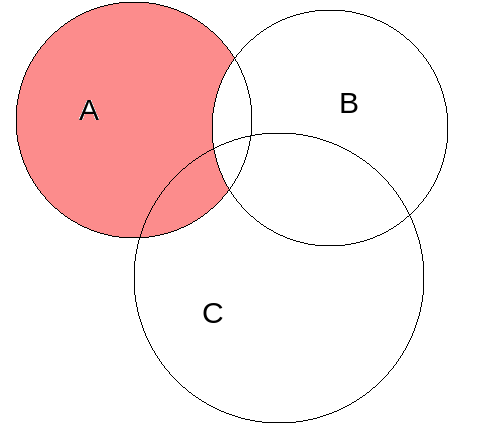
\includegraphics[width=50mm]{images/1.png}
    
    \item $(C \cup B) \bigtriangleup A$
    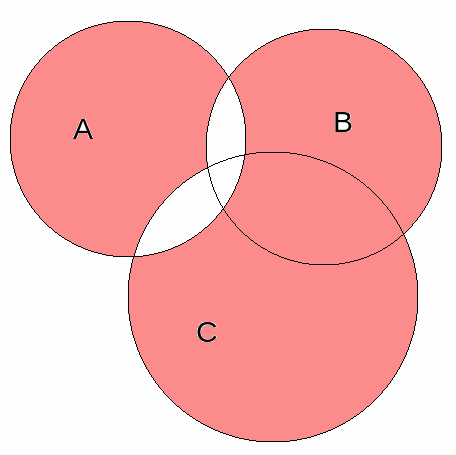
\includegraphics[width=50mm]{images/2.png}
\end{enumerate}

\noindent\makebox[\linewidth]{\rule{\paperwidth}{0.4pt}}

$$Y = (B \bigtriangleup (A \bigtriangleup C)) \bigtriangleup (B \cap C)$$ 

\begin{enumerate}
    \item $(A \bigtriangleup C)$
    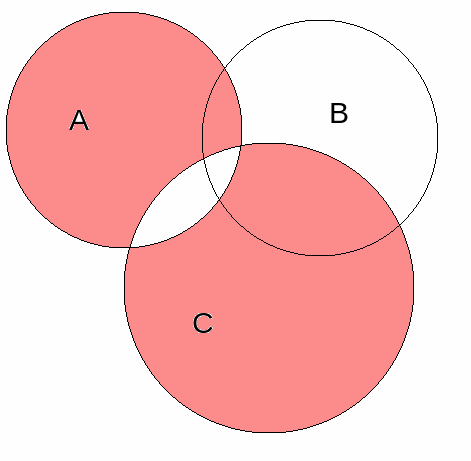
\includegraphics[width=50mm]{images/3.png}
    
    \item $(B \bigtriangleup (A \bigtriangleup C))$
    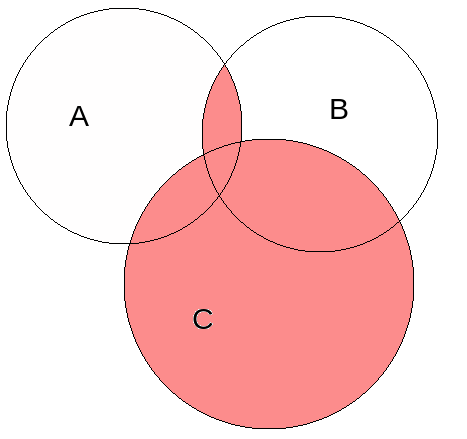
\includegraphics[width=50mm]{images/4.png}
    
    \item $(B \cap C)$
    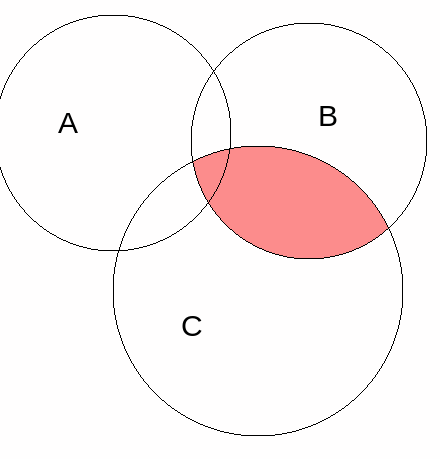
\includegraphics[width=50mm]{images/5.png}
    
    \item $(B \bigtriangleup (A \bigtriangleup C)) \bigtriangleup (B \cap C)$
    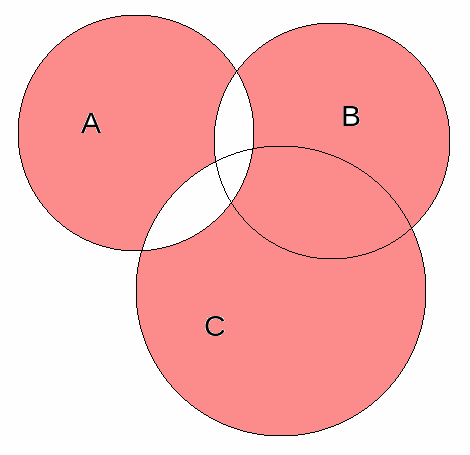
\includegraphics[width=50mm]{images/6.png}
\end{enumerate}

\noindent\makebox[\linewidth]{\rule{\paperwidth}{0.4pt}}

$$Y = A \setminus \overline{(B \cup (C \setminus (B \cap A)))}$$

\begin{enumerate}
    \item $(B \cap A)$
    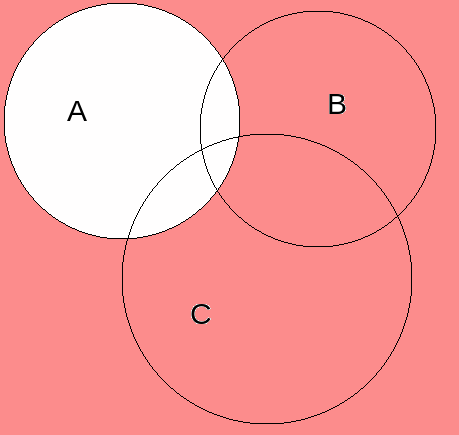
\includegraphics[width=50mm]{images/7.png}
    
    \item $(C \setminus (B \cap A))$
    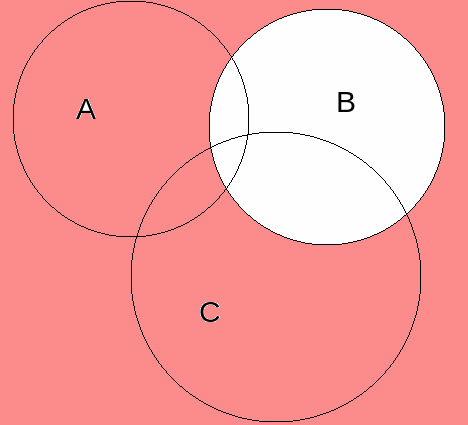
\includegraphics[width=50mm]{images/8.png}
    
    \item $(B \cup (C \setminus (B \cap A)))$
    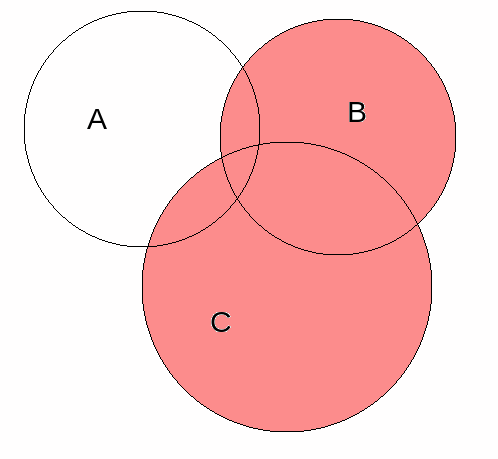
\includegraphics[width=50mm]{images/9.png}
    
    \item $\overline{(B \cup (C \setminus (B \cap A)))}$
    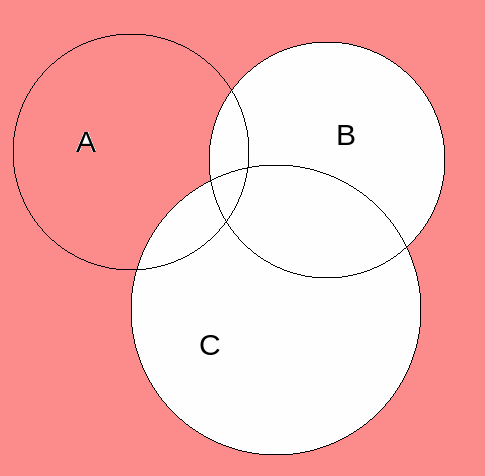
\includegraphics[width=50mm]{images/10.png}
    
     \item $ A \setminus \overline{(B \cup (C \setminus (B \cap A)))}$
    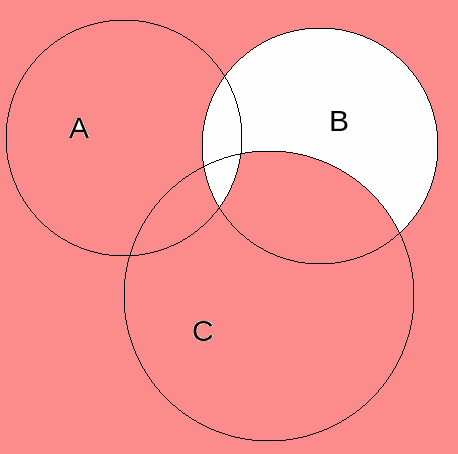
\includegraphics[width=50mm]{images/11.png}
\end{enumerate}

\noindent\makebox[\linewidth]{\rule{\paperwidth}{0.4pt}}

$$Y = (C \bigtriangleup (A \bigtriangleup (C \bigtriangleup B))) \cup A$$

\begin{enumerate}
    \item $(C \bigtriangleup B)$
    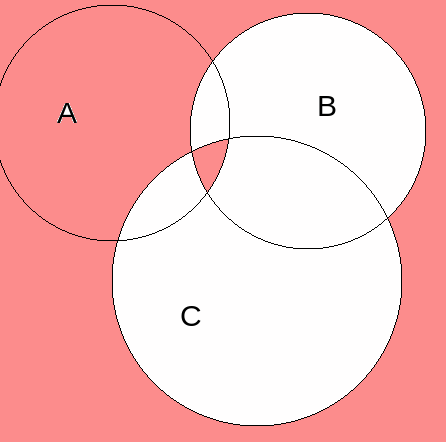
\includegraphics[width=50mm]{images/12.png}
    
    \item $(A \bigtriangleup (C \bigtriangleup B))$
    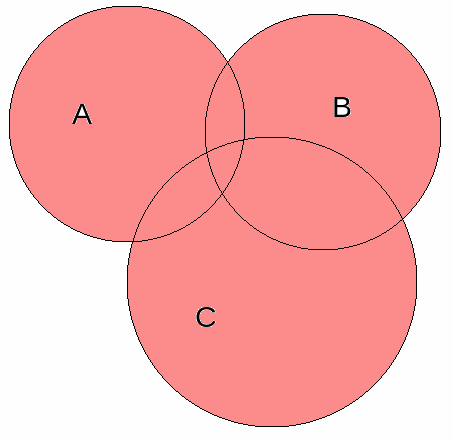
\includegraphics[width=50mm]{images/13.png}
    
    \item $(C \bigtriangleup (A \bigtriangleup (C \bigtriangleup B)))$
    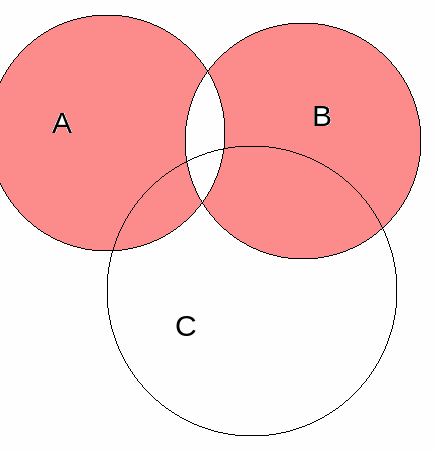
\includegraphics[width=50mm]{images/14.png}
    
    \item $(C \bigtriangleup (A \bigtriangleup (C \bigtriangleup B))) \cup A$
    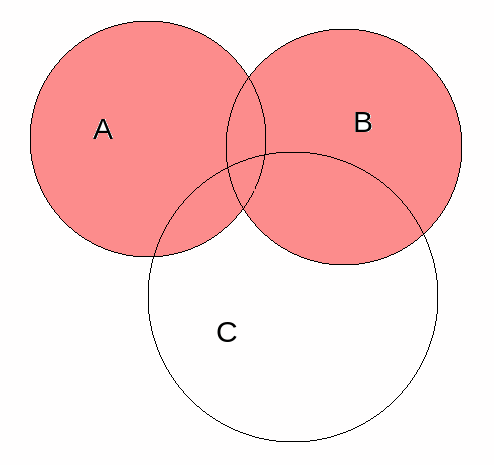
\includegraphics[width=50mm]{images/15.png}
    
\end{enumerate}

\noindent\makebox[\linewidth]{\rule{\paperwidth}{0.4pt}}

$$Y = (\overline{(B \cap C)} \setminus A) \cap (B \setminus C)$$

\begin{enumerate}
    \item $(B \cap C)$
    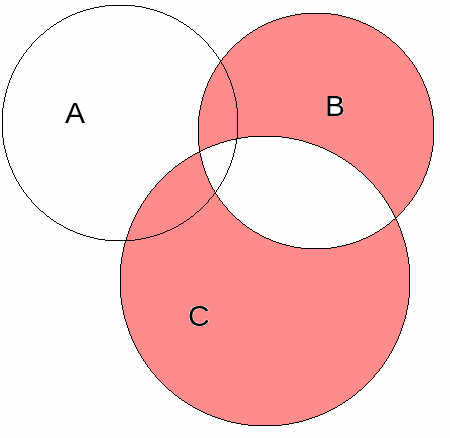
\includegraphics[width=50mm]{images/16.png}
    
    \item $\overline{(B \cap C)}$
    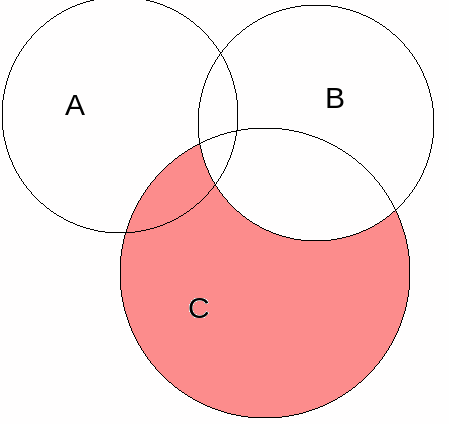
\includegraphics[width=50mm]{images/17.png}
    
    \item $(\overline{(B \cap C)} \setminus A)$
    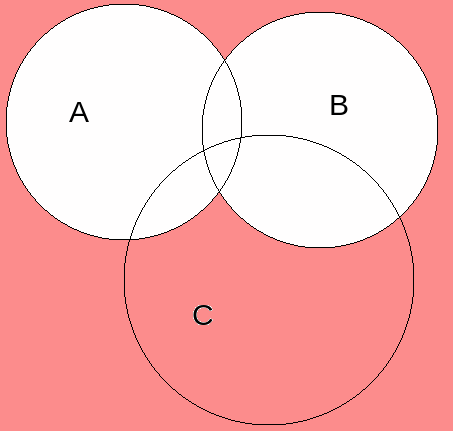
\includegraphics[width=50mm]{images/18.png}
    
    \item $(B \setminus C)$
    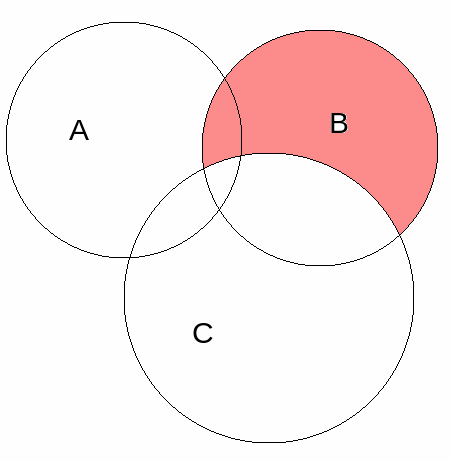
\includegraphics[width=50mm]{images/19.png}
    
    \item $(\overline{(B \cap C)} \setminus A) \cap (B \setminus C)$
    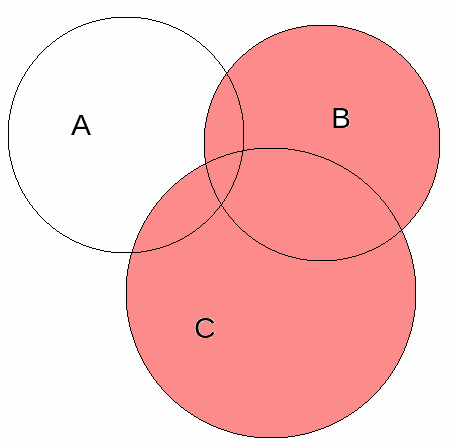
\includegraphics[width=50mm]{images/21.png}
\end{enumerate}

\noindent\makebox[\linewidth]{\rule{\paperwidth}{0.4pt}}

$$Y = ((C \bigtriangleup B) \cup C) \bigtriangleup (A \setminus B)$$

\begin{enumerate}
    \item $(C \bigtriangleup B)$
    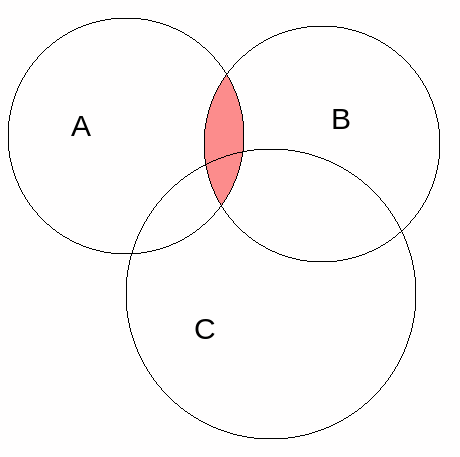
\includegraphics[width=50mm]{images/22.png}
    
    \item $((C \bigtriangleup B) \cup C)$
    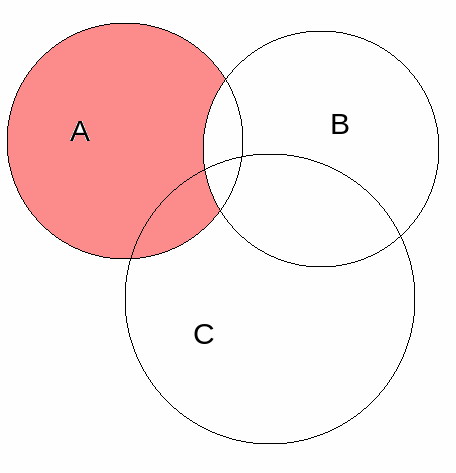
\includegraphics[width=50mm]{images/23.png}
    
    \item $(A \setminus B)$
    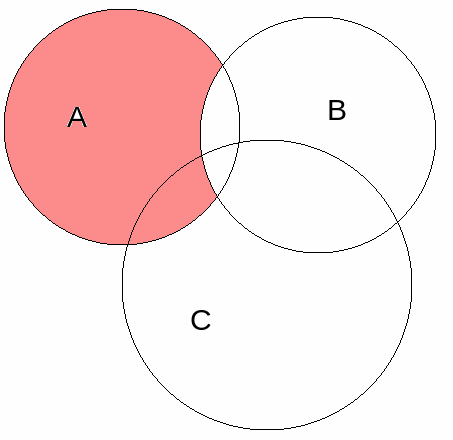
\includegraphics[width=50mm]{images/24.png}
    
    \item $((C \bigtriangleup B) \cup C) \bigtriangleup (A \setminus B)$
    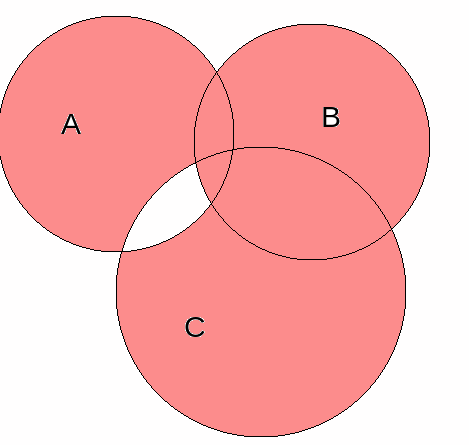
\includegraphics[width=50mm]{images/25.png}
\end{enumerate}

\noindent\makebox[\linewidth]{\rule{\paperwidth}{0.4pt}}

\end{document}
